% !TeX root = ../../../main.tex
\begin{figure}[!ht]

\centering
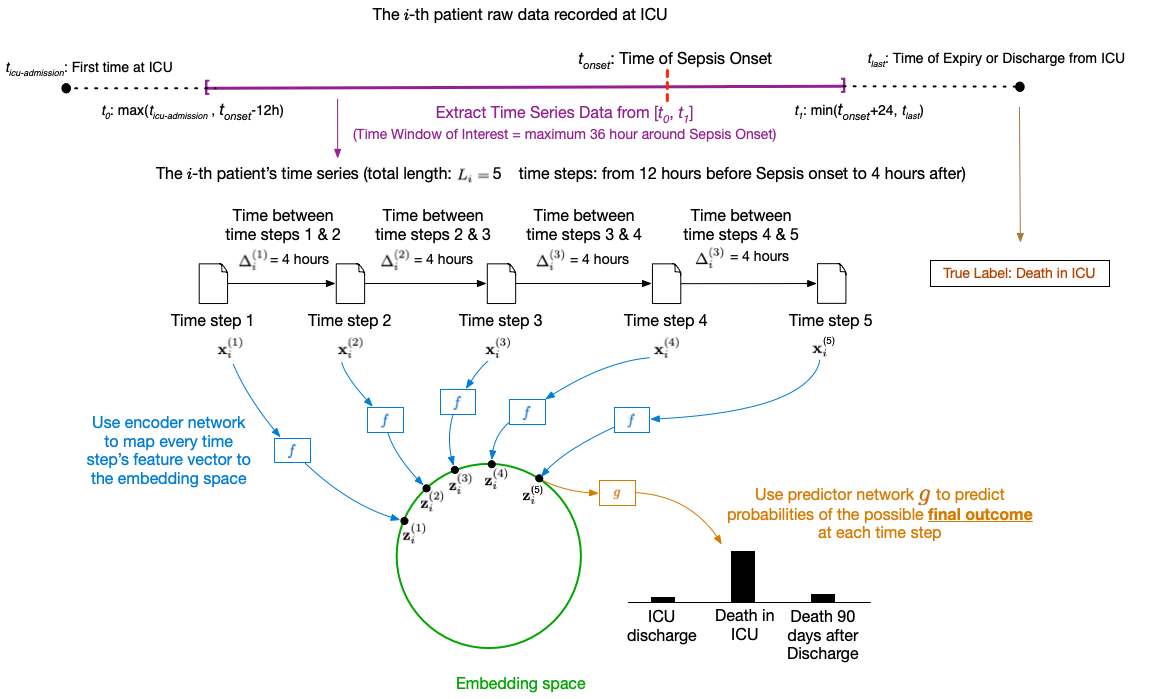
\includegraphics[width=.99\linewidth]{Appendices/appendix-ch02/images/MIMIC-Setup.png}
%\vspace{-2.5em}
 \caption{Setup for MIMIC Experiments at Inference time from \ChTwoSmallCaps{Temporal-SCL}: First, we extract time series data for each patient from a time window around their sepsis onset within their complete ICU data timeline. This time series data is transformed into multiple time steps at 4-hour intervals. The resulting time series will have its features at each time step mapped onto the embedding space learned by our encoder. Finally, these resulting embeddings will be passed through our predictor network to predict the ICU mortality of each patient at every time step.
 %\vspace{-1em}
 }   \ChTwoFloatLabel{ch02:fig:mimic-setup}
\end{figure}